\section{Introduction}
Given a non-empty set $\mathcal{A}$, a partition $\Pi$ of $\mathcal{A}$ is defined as a collection of subsets of $\mathcal{A}$, i.e., $\Pi = \{A_1, A_2, \ldots, A_k\}$, such that:

\begin{itemize}
    \item $\bigcup\limits_{i = 1}^{k} A_i = \mathcal{A}$.
    \item $A_i \cap A_j = \emptyset$ for all $i \neq j$.
\end{itemize}

The elements of $\Pi$ are called \textit{classes}. Furthermore, we define an equivalence relation between two elements $a, b \in \mathcal{A}$ by stating that $a$ and $b$ are equivalent if and only if there exists some $A_i \in \Pi$ such that $a, b \in A_i$. In this case, we say that $a$ and $b$ are equivalent and denote this by $a \equiv b$.

One can trivially verify that this binary relation is reflexive, symmetric, and transitive. These properties allow us to define a \textit{representative} for each class—an element that represents the entire class. By the reflexive, symmetric, and transitive properties, every other element in the same class is related to this \textit{representative}.

This concept, previously established by mathematicians, is widely used in Computer Science to implement the Union-Find data structure. The Union-Find data structure is designed to efficiently store and manage a partition of a set $\mathcal{A}$. It provides two fundamental operations:

\begin{itemize}
    \item \texttt{Find Operation:} Given an element $a \in \mathcal{A}$ find the representative of the class from which $a$ belongs.
    \item \texttt{Union Operation:} Given two element $a \in A_i$ and $b \in A_j$ make a union of classes $A_i$ and $A_j$. That is, if the Union-Find represents a partition $\Pi$, after doing the \texttt{Union} operation the data structure will represent a new partition $\Pi'$ such that $\Pi' =  (\Pi \setminus \{A_i,A_j\}) \cup (\{A_i \cup A_j\})$
\end{itemize}

\section{Implementation}
A C++ implementation has been made for the sake of efficiency of the Union-Find operations. A C++ class has been created for the Union-Find data structure (look at \texttt{UnionFind.hh} for a more detailed exploration of the class). It consists mainly of an array in which every element will either point to another element that belongs to the same class or it will be the representative. For the representative, depending on the union strategy they will be represented differently:

\begin{itemize}
    \item With the Quick-Union strategy an element $i$ is the representative of a class if $v[i] = i$.
    \item With the other strategies (union by rank/size) they will be represented by a negative number that indicates the size/rank multiplied by $-1$ (i.e. $v[i] = -size$ or $v[i] = -rank$).
\end{itemize}

The \texttt{main.cc} file requires, as input, the size of the data structure, a Union strategy (a natural number between 0 and 2, representing Quick-Union, Union by Weight, and Union by Rank, respectively), and a Path strategy (a natural number between 0 and 4, representing No Compression, Full Compression, Path Splitting, Path Halving and Type One Reversal (a new heuristic explained later)). After that, the program will repeatedly request two natural numbers (the elements to be merged) and perform the corresponding union operation. This process continues until the data structure consists of a single block, at which point the program terminates.

Every $\Delta = 250$ elements, the program will output information about the current TPL and TPU of the data structure. The TPU parameter is computed using a counter that increments by one each time a pointer switch occurs (see Appendix \ref{ap:Path}), while the TPL is calculated by traversing the entire data structure (see Appendix \ref{ap:TPL}). Although this approach may not be the most efficient in terms of performance, the author chose this method for computing the TPL because the focus is on obtaining the value rather than optimizing execution time. Later, execution time will be measured separately, excluding this part of the computation.

To execute the program, one can compile it using the provided \texttt{Makefile} by running \texttt{make main} and then executing the program from the command line. For instance, suppose \texttt{file.txt} contains pairs of numbers (between 0 and 999) that, when processed, will lead to a single block in the Union-Find data structure. In that case, we can process these numbers using Union by Weight and Path Halving by executing the following command:

\texttt{./main.exe 1000 1 3 < file.txt}

For getting time results you just need to compile by running \texttt{make main\_time}.

\section{Experimental Setup}
To generate random instances, a number \( n \) of elements and a seed \( s \) are requested as input. Then, this program generates a random number of different pairs \( (i, j) \) where \( 0 \leq i < j < n \) until the total number of pairs generated forms a single block in a Union-Find data structure. 

The time complexity of this program is difficult to calculate, as there is no guarantee that the program will terminate. Since it generates pseudo-random different pairs, it might enter a loop where all the pairs generated are repetitions. However, this approach is better than the initial implementation, which involved generating all possible \(n \choose 2 \) pairs—requiring \( \Theta(n^2) \) time and space complexity—and then selecting random pairs until a single block is formed in the Union-Find structure. Using this new approach we use a \texttt{C++ set} to keep track of all different pairs, requesting only necessary memory.

For the following experiments, $20$ instances of size ($n = 1000, 5000, 10000$) have been created. Each instance was generated with a seed $s$ that goes from $1964$ (in honor of Union-Find data structure discover\cite{galler1964improved}!) to $1983$. Each instance has been executed with the $15$ possible different strategies and the data has been collected as follows:

\begin{enumerate}
    \item For each size \( n \), union strategy, and path strategy, execute all instances of size \( n \).
    \item We will average all values obtained for every \( k \in \{\Delta, 2\Delta, 3\Delta, \ldots\} \) pairs processed of all instances with same size and heuristics, provided that at least five instances have reached the point of processing \( k \) pairs.
\end{enumerate}

Although this process might be tedious, it can be automated by executing a single script! (See README).

Using these samples, we were able to process approximately 3,750 pairs of elements for \( n = 1000 \), 26,250 pairs for \( n = 5000 \), and 52,250 pairs for \( n = 10,000 \).  

\section{Results}
\subsection{Metric Comparisons}
\subsubsection{Path Strategy: No Compression}
Using this technique, the minimization of paths between an element \( i \) and its representative \( r_i \) relies solely on the Union heuristic. Specifically, in the case of Quick-Union, Figure \ref{fig:tplNC} shows that Quick-Union differs significantly from TPL compared to the other union techniques. This difference is expected, as no heuristic is used to minimize these paths.  

In fact, since the total path length is significantly larger when not using unions with heuristics, we can be certain that the asymptotic cost will be much higher. Indeed, although \texttt{union} operations are \( \Theta(1) \), a \texttt{find} operation can theoretically take as much as \( \Theta(n) \). However, we observe that the TPL stabilizes after approximately 50\% of the pairs have been processed.  

This is not surprising because, as more unions are performed, the probability that the selected pair is already connected increases, meaning the union operation has no effect and the TPL remains unchanged. Still, we can see that the TPL increases as $n$ increases. 

Taking a closer look at unions with heuristics, which are also shown in Figure \ref{fig:tplNC}, we observe two key differences compared to Quick-Union:  
\begin{itemize}  
    \item TPL stabilizes sooner than in Quick-Union. Specifically, it reaches a \textit{constant} value of approximately 2 after processing around 20\%–30\% of the pairs.  
    \item Although TPL increases slightly as \( n \) grows, it consistently remains close to 2. In fact from a theoretical analysis we know that a block of size $k$ has $O(\log k)$ height using these unions, which also helps to explain why we reach this stability \textit{sooner}. This indicates that using heuristics in unions leads to overall stability in TPL and, consequently, in \texttt{find} operations. 
\end{itemize}  

Between Union by Weight/Size, there is no significant difference between the two strategies, although Union by Size performs slightly better. However, both strategies significantly outperform Quick-Union without any path compression technique.

\begin{figure}[ht]
    \centering
    % Subfigure 1
    \begin{subfigure}{0.32\textwidth}
        \centering
        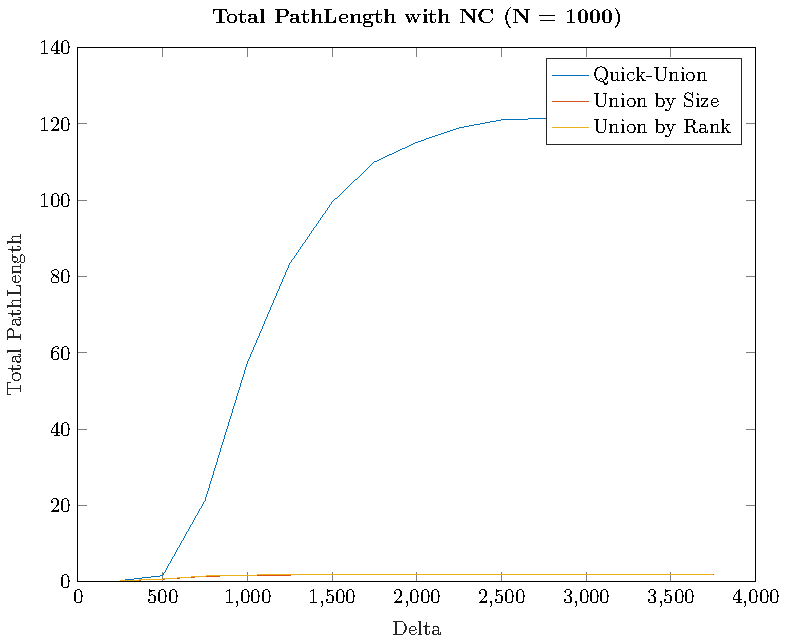
\includegraphics[width=\textwidth]{../images/plotNCFull1000_PathLength.pdf}
        \caption{Path Lengths with different union strategies with $n = 1000$}
    \end{subfigure}%
    \hfill
    % Subfigure 2
    \begin{subfigure}{0.32\textwidth}
        \centering
        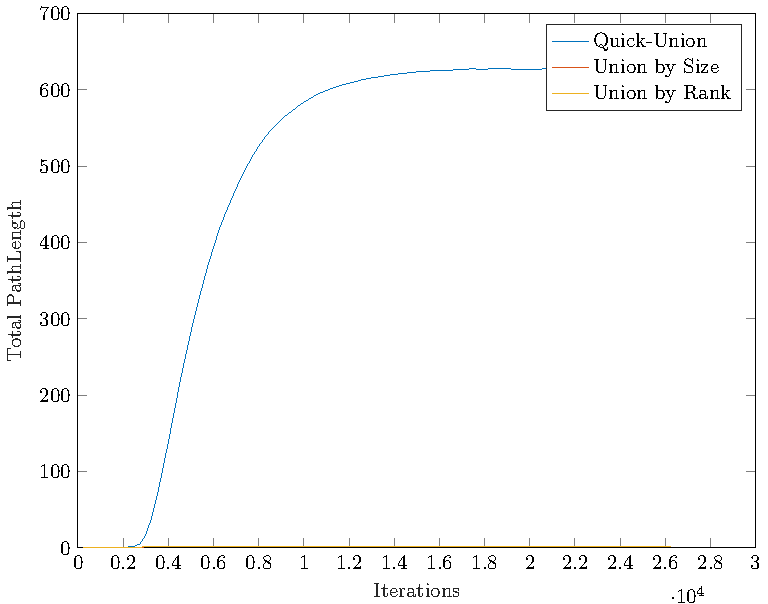
\includegraphics[width=\textwidth]{../images/plotNCFull5000_PathLength.pdf}
        \caption{Path Lengths with different union strategies with $n = 5000$}
    \end{subfigure}%
    \hfill
    % Subfigure 3
    \begin{subfigure}{0.32\textwidth}
        \centering
        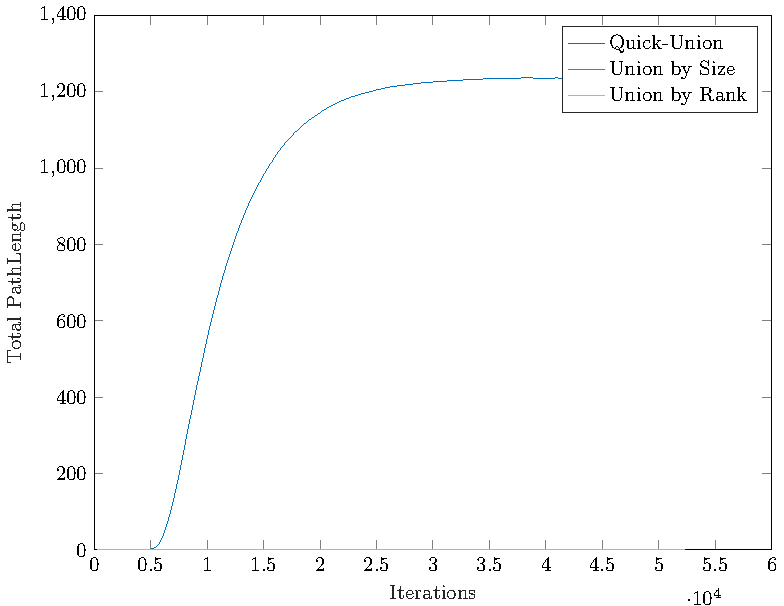
\includegraphics[width=\textwidth]{../images/plotNCFull10000_PathLength.pdf}
        \caption{Path Lengths with different union strategies with $n = 10000$}
    \end{subfigure}

    \caption{Total Path Length normalized with No Compression}
    \label{fig:tplNC}
\end{figure}

\begin{figure}[ht]
    \centering
    % Subfigure 1
    \begin{subfigure}{0.32\textwidth}
        \centering
        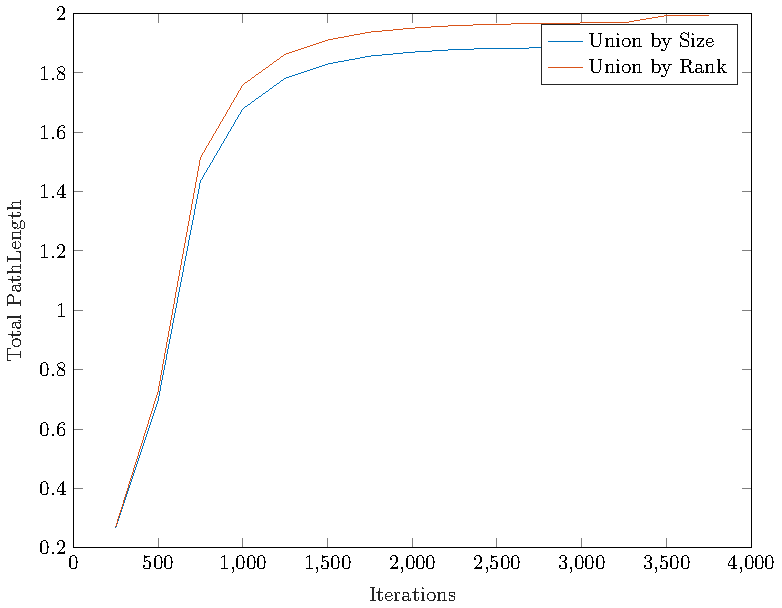
\includegraphics[width=\textwidth]{../images/plotNCNonFull1000_PathLength.pdf}
        \caption{Path Lengths with different union strategies with $n = 1000$}
    \end{subfigure}%
    \hfill
    % Subfigure 2
    \begin{subfigure}{0.32\textwidth}
        \centering
        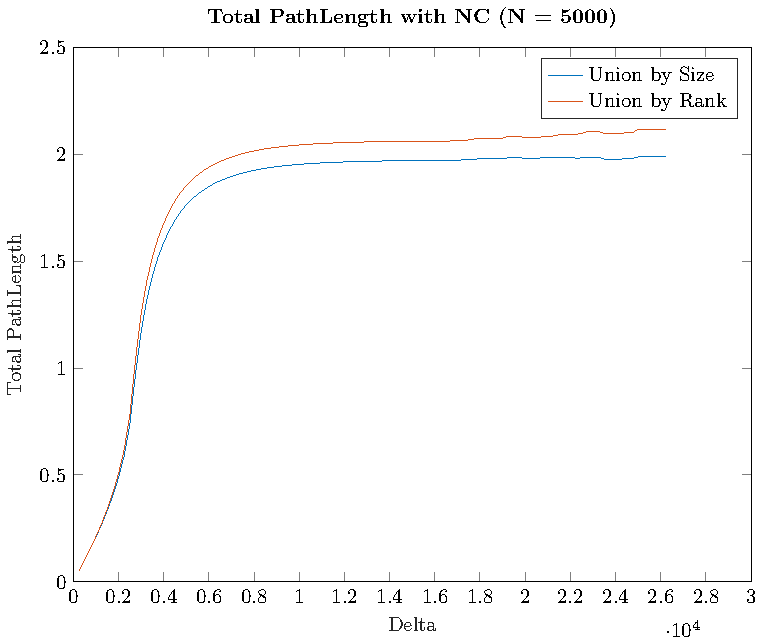
\includegraphics[width=\textwidth]{../images/plotNCNonFull5000_PathLength.pdf}
        \caption{Path Lengths with different union strategies with $n = 5000$}
    \end{subfigure}%
    \hfill
    % Subfigure 3
    \begin{subfigure}{0.32\textwidth}
        \centering
        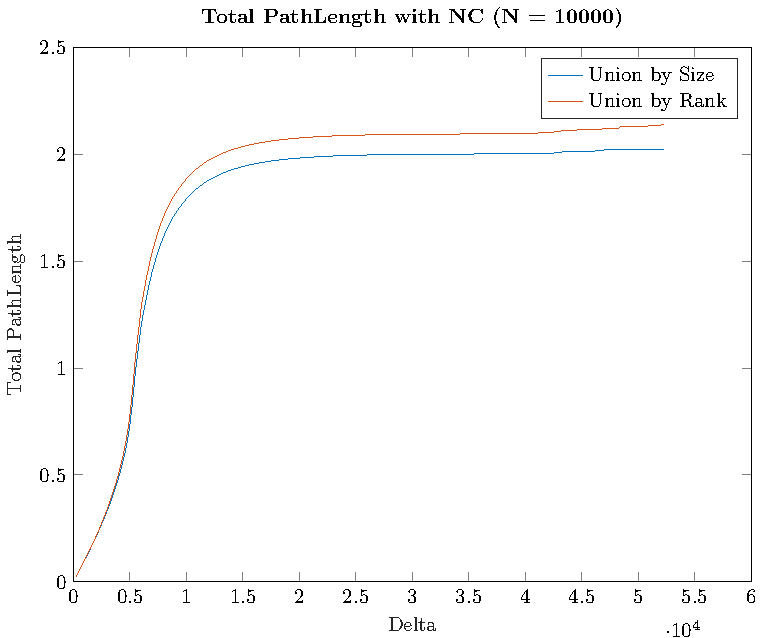
\includegraphics[width=\textwidth]{../images/plotNCNonFull10000_PathLength.pdf}
        \caption{Path Lengths with different union strategies with $n = 10000$}
    \end{subfigure}

    \caption{Total Path Length normalized with No Compression without Quick-Union}
    \label{fig:tplNCNoQU}
\end{figure}




\subsubsection{Path Strategy: using Heuristics}

Now let us introduce \textit{Path Compression} in our analysis. This technique consists in, when a \texttt{find} operation is performed, rearranging pointers so that we expect that future \texttt{find} operations take less time. In this analysis we are going to consider the following path compression heuristics:

\begin{itemize}
    \item The \textbf{Full Compression} heuristic ensures that every element in the path from \( i \) to the representative of the class \( r_i \) will point directly to \( r_i \) by traversing the path twice (first to identify \( r_i \) and second to rearrange the pointers). At the cost of traversing this path twice, we expect to speed up future find operations involving a class where this heuristic has been applied. 
    \item Traversing a path twice might not always be the best option so, in order to speed up future find operations, we are going to decrement path lengths within the class by making that every node points to its grandparent as long as this exists. That is what \textbf{Path Splitting} and \textbf{Path Halving} does. The only difference between Path Splitting and Halving is that in splitting we will always make every node point to its grandparent (as long as they exists) while in halving we are going to do that operation every other node (so we expect to end sooner a find operation).
    \item Similar to Full Compression we have \textbf{Type One Reversal} which, given a path $(i, n_1, n_2, \ldots, n_k, r_i)$ where $i$ is an element and $r_i$ is its representative, consists of the following: Every node from $n_1$ up to $n_k$ will point to $i$ and $i$ will point to $r_i$. Although this might be strange, this heuristic has a similar idea to Full Compression but this time we are traverse a path only once instead of twice at the cost of not pointing directly to the representative. In this analysis we will only consider \textbf{Type One Reversal} but in \cite{tarjan1984worst} is defined a type $k$ reversal for $k \geq 1$.
\end{itemize}

As expected, we see in Figure \ref{fig:tplH} that Quick-Union, once again, performs the worst. However, this time, full compression, path splitting, and path halving exhibit similar behavior in terms of TPL: it initially grows quickly but soon tends to converge to the TPL achieved using unions with heuristics.  

Again, this should not be surprising, as increasing the number of iterations raises the probability that two pairs belong to the same class. For knowing if two elements belong to the same class we need to perform two \texttt{find} operations, and when these operations are executed with compression heuristics, they tend to \textit{fix} paths within the trees, thereby reducing the IPL corresponding to the tree of such class.

Although full compression, splitting, and halving perform very similarly, we observe slight differences in the maximum peak of the TPL. In fact, the more compression applied in the heuristic, the lower the peak values become, though the difference remains unnoticeable in practice.

Still, it is interesting to examine Type One Reversal. Unlike previous heuristics, it does not converge to the TPL obtained with unions with heuristics; instead, it remains closer to a value approximately twice the peak values observed with other compression heuristics.  

Type One Reversal is a tricky compression heuristic because performing a \texttt{find} operation in a class may result in a new tree representation with a higher internal path length than before the operation. For instance see Figure \ref{fig:torIPL}, where we decreased by one the path lengths of all subtrees rooted at node 4, but simultaneously increased by one the path lengths of all subtrees rooted at node 3.  


\begin{figure}[ht]
    \centering
    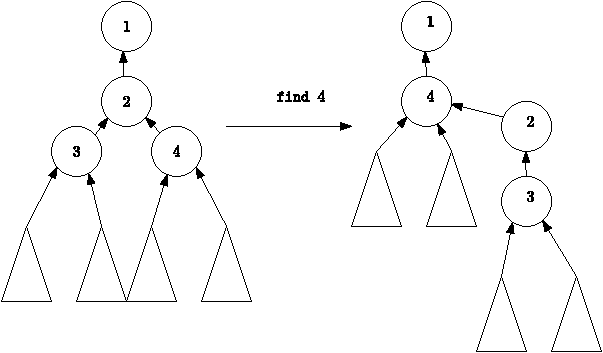
\includegraphics[scale=0.95]{../images/tor.pdf}
    \caption{Example of Type One Reversal which may lead to a worst IPL}
    \label{fig:torIPL}
\end{figure}

In fact, when Quick-Union with Type One Reversal reaches a \textit{stable} point in total path length, it continuously improves and deteriorates in an oscillatory manner.  

A more general view of Figure \ref{fig:torIPL} can be found in Figure \ref{fig:torEx}, where we start with a generic tree configuration using this path compression technique. This configuration consists of a representative, a single node pointing to the representative, and several subtrees pointing to this intermediate node.  

In Figure \ref{fig:torEx}, we illustrate a \texttt{find} operation that is always performed at the root of a subtree. If this was not initially the case, the node would become the root of the subtree after applying compression, ensuring that our representation remains valid. Additionally, we depict nodes 3 and 4 as having only two subtrees pointing to them. This simplification is solely for clarity in the figure; in reality, each node may have a different number of subtrees pointing to it.  

\begin{figure}[ht]
    \centering
    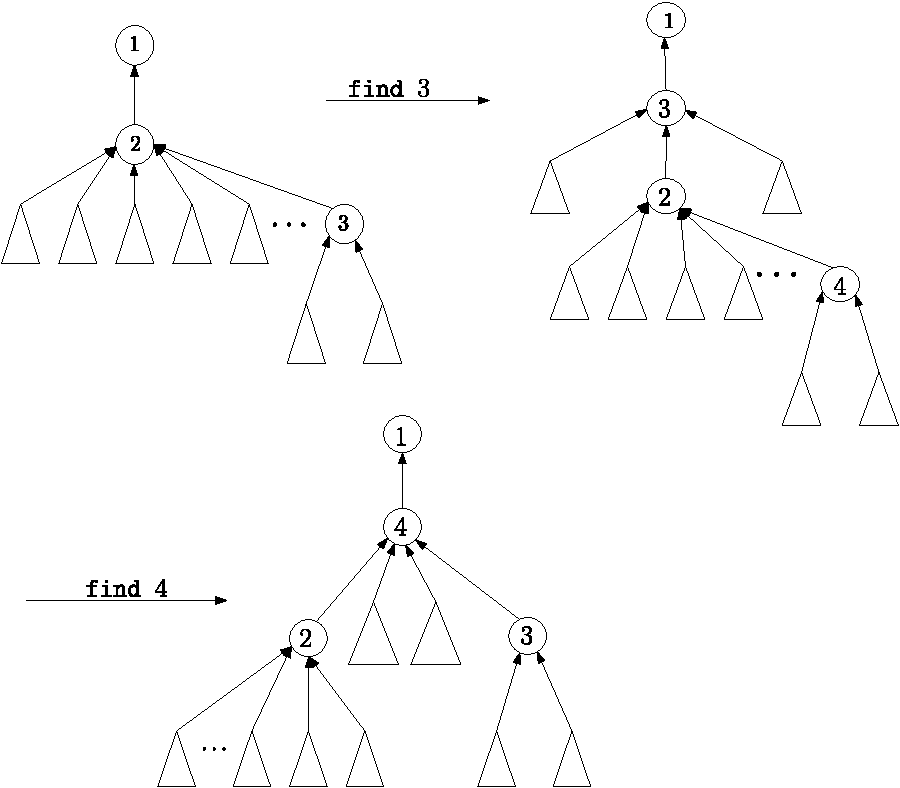
\includegraphics[scale=0.65]{../images/torEx.pdf}
    \caption{More accurate example of the representation of a tree after several \texttt{find} operations}
    \label{fig:torEx}
\end{figure}

Now we see that performing a \texttt{find} operation will increase by one the distance of all nodes in a subtree to the representative while decreasing by one the distance in another subtree.

If we apply union heuristics, due to this adjustment and the randomness introduced in our analysis, each subtree will have approximately the same number of nodes. Consequently, when performing another \texttt{find} operation, it is more likely to occur in a node within the subtree rooted at $2$ rather than any other node. As a result, we will then increase by one the distance of each node in the subtree rooted at $3$ to the representative while decreasing by one the distance in the subtree rooted at $4$. 

In fact, this behavior is observed in Figure \ref{fig:tpuNH}, where the TPL remains between $2$ and $3$. If we do not attempt to balance each tree in the union heuristics, we may end up increasing the distance for more nodes than we decrease, potentially by one or even more.

Regarding pointer updates (Figures \ref{fig:tpuH} and \ref{fig:tpuNH}), we highlight the following observations:

\begin{itemize}
    \item Full Compression and Path Splitting perform a similar number of pointer updates, which is expected since all nodes along the same path will have their pointers updated.
    \item Path Halving performs slightly fewer pointer updates, which makes sense as it updates pointers for every other node.
    \item Type One Reversal always increases the number of pointer updates, as it consistently modifies pointers.
    \item The longer a path is, the more pointer updates are required. This explains why Quick-Union consistently performs the worst.
\end{itemize}

\begin{figure}[ht]
    \centering
    \begin{subfigure}{0.32\textwidth}
        \centering
        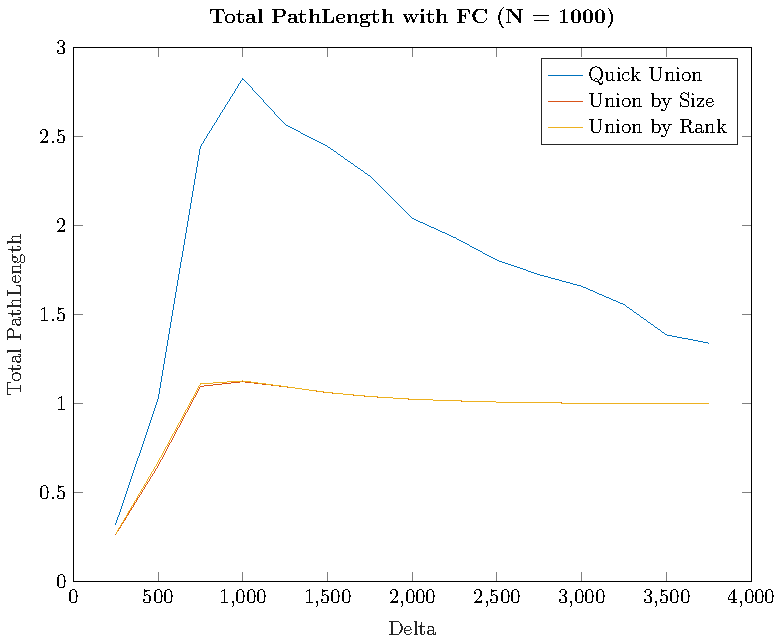
\includegraphics[width=\textwidth]{../images/plotFCFull1000_PathLength.pdf}
        \caption{Path Lengths with different union strategies with $n = 1000$ using Full Compression}
    \end{subfigure}%
    \hfill
    % Subfigure 2
    \begin{subfigure}{0.32\textwidth}
        \centering
        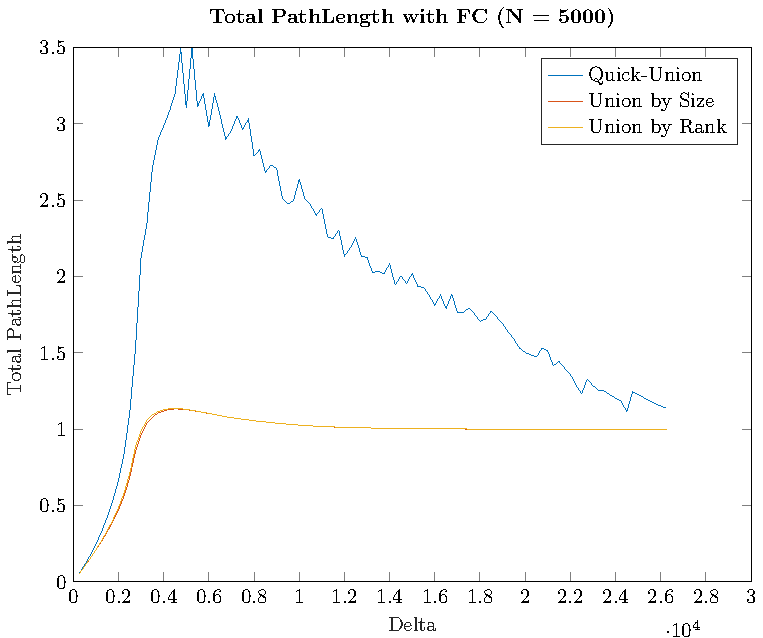
\includegraphics[width=\textwidth]{../images/plotFCFull5000_PathLength.pdf}
        \caption{Path Lengths with different union strategies with $n = 5000$ using Full Compression}
    \end{subfigure}%
    \hfill
    % Subfigure 3
    \begin{subfigure}{0.32\textwidth}
        \centering
        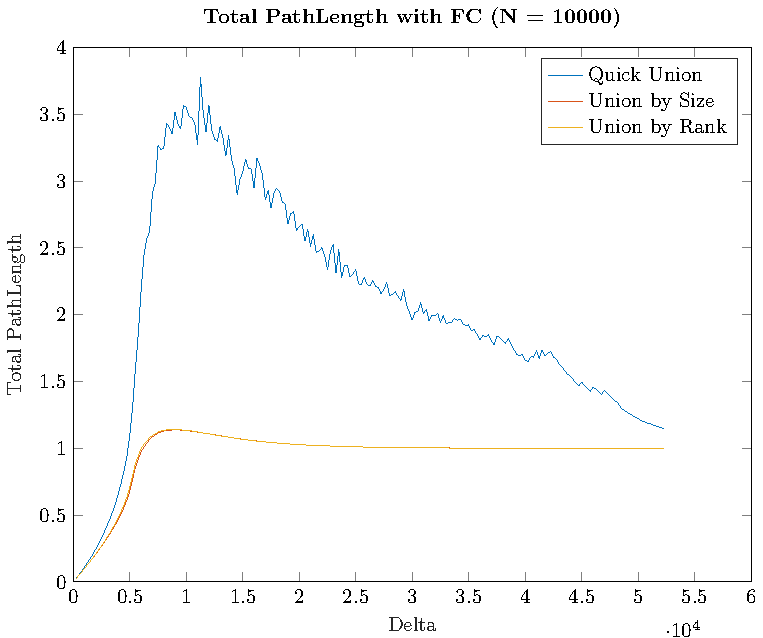
\includegraphics[width=\textwidth]{../images/plotFCFull10000_PathLength.pdf}
        \caption{Path Lengths with different union strategies with $n = 10000$ using Full Compression}
    \end{subfigure}
    % Subfigure 1
    \begin{subfigure}{0.32\textwidth}
        \centering
        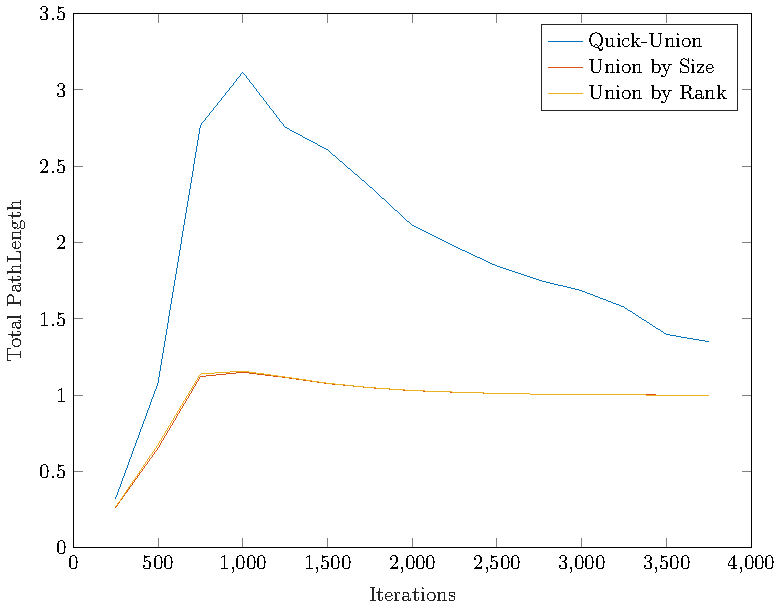
\includegraphics[width=\textwidth]{../images/plotPSFull1000_PathLength.pdf}
        \caption{Path Lengths with different union strategies with $n = 1000$ using Path Splitting}
    \end{subfigure}%
    \hfill
    % Subfigure 2
    \begin{subfigure}{0.32\textwidth}
        \centering
        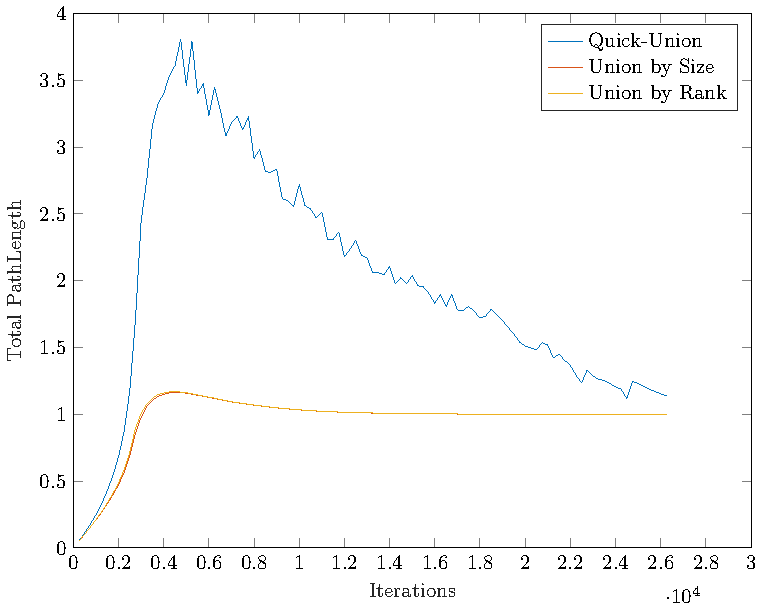
\includegraphics[width=\textwidth]{../images/plotPSFull5000_PathLength.pdf}
        \caption{Path Lengths with different union strategies with $n = 5000$ using Path Splitting}
    \end{subfigure}%
    \hfill
    % Subfigure 3
    \begin{subfigure}{0.32\textwidth}
        \centering
        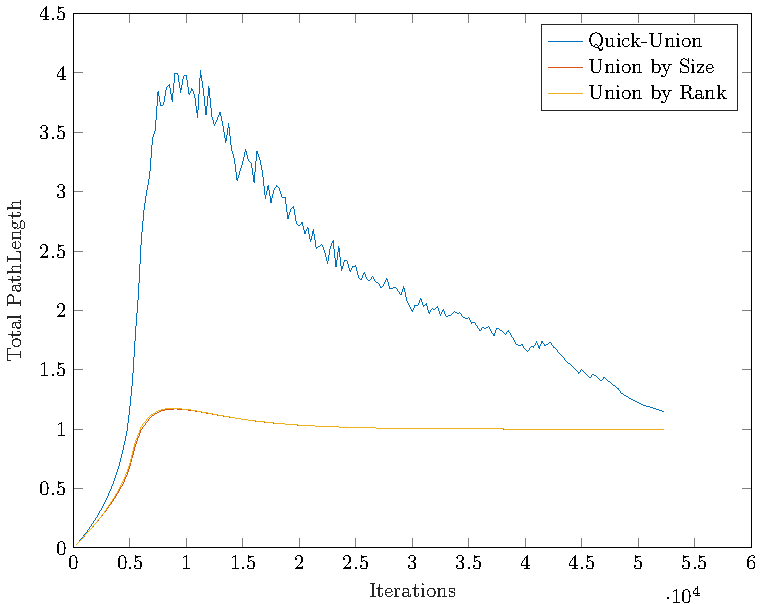
\includegraphics[width=\textwidth]{../images/plotPSFull10000_PathLength.pdf}
        \caption{Path Lengths with different union strategies with $n = 10000$ using Path Splitting}
    \end{subfigure}

    \begin{subfigure}{0.32\textwidth}
        \centering
        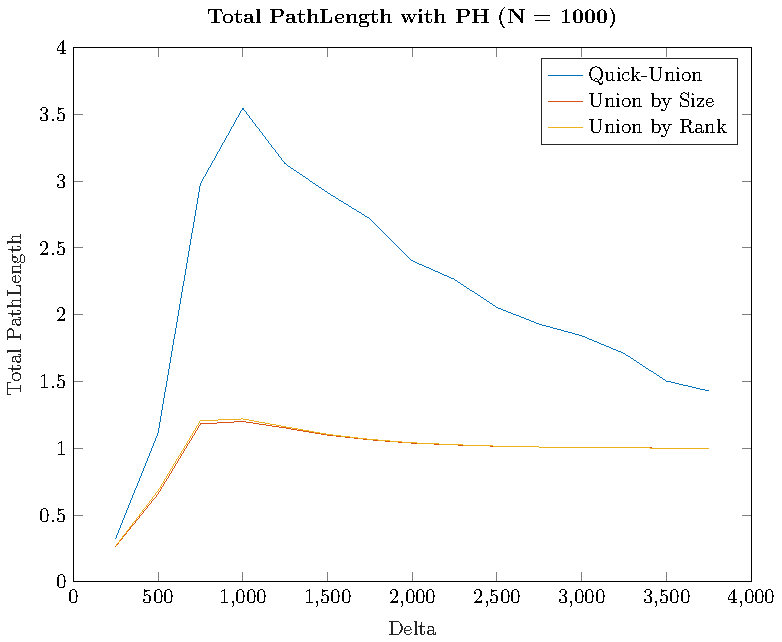
\includegraphics[width=\textwidth]{../images/plotPHFull1000_PathLength.pdf}
        \caption{Path Lengths with different union strategies with $n = 1000$ using Path Halving}
    \end{subfigure}%
    \hfill
    % Subfigure 2
    \begin{subfigure}{0.32\textwidth}
        \centering
        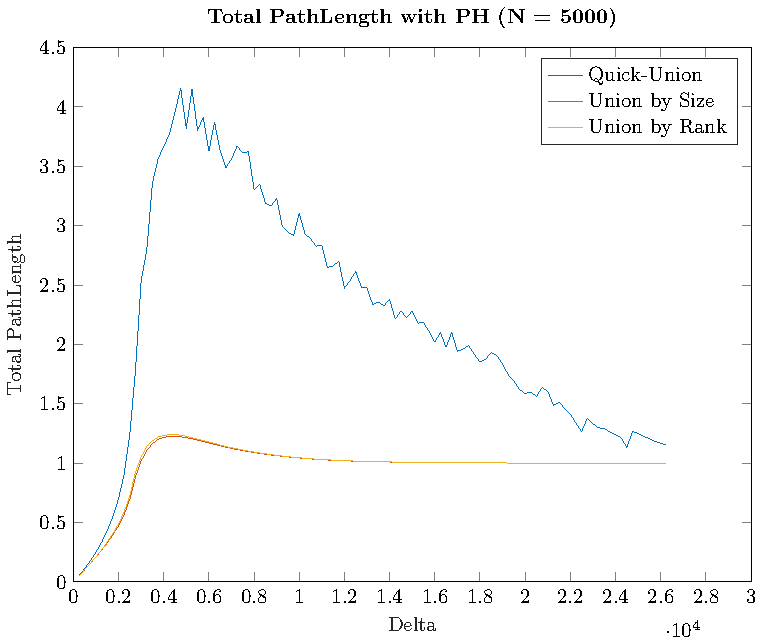
\includegraphics[width=\textwidth]{../images/plotPHFull5000_PathLength.pdf}
        \caption{Path Lengths with different union strategies with $n = 5000$ using Path Halving}
    \end{subfigure}%
    \hfill
    % Subfigure 3
    \begin{subfigure}{0.32\textwidth}
        \centering
        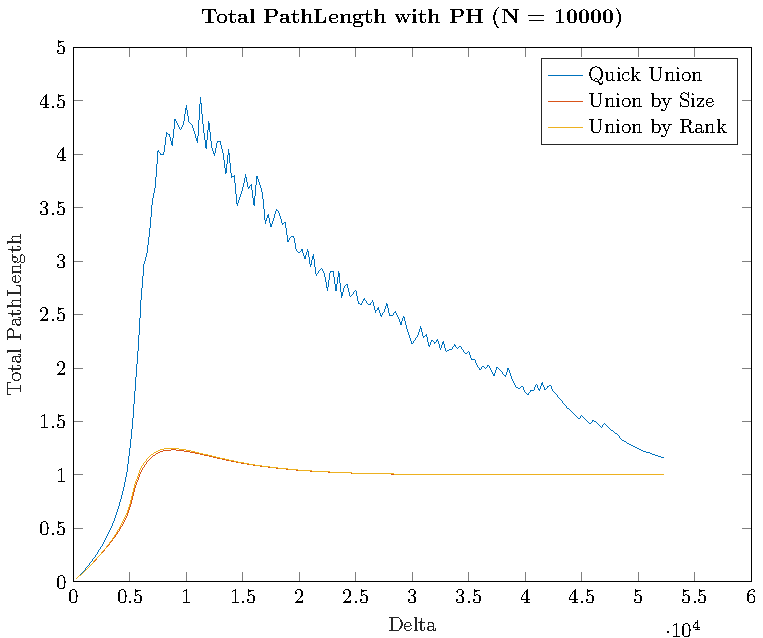
\includegraphics[width=\textwidth]{../images/plotPHFull10000_PathLength.pdf}
        \caption{Path Lengths with different union strategies with $n = 10000$ using Path Halving}
    \end{subfigure}

    \begin{subfigure}{0.32\textwidth}
        \centering
        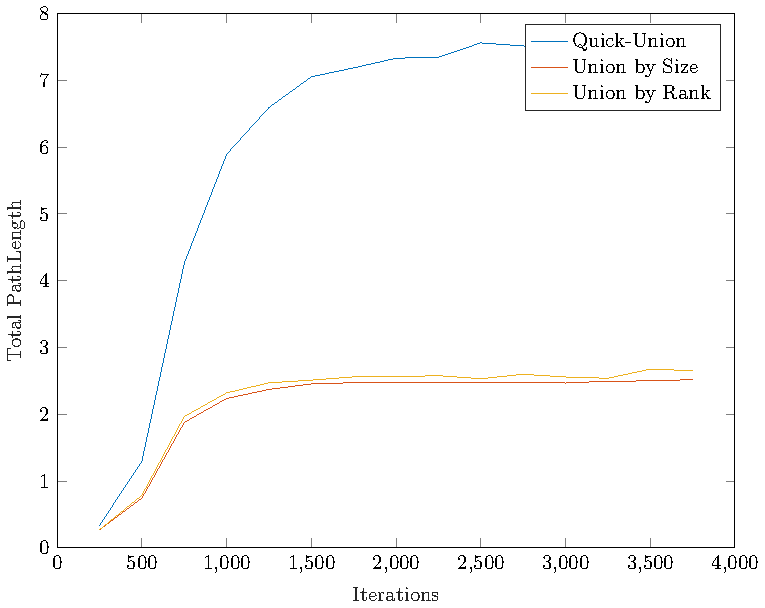
\includegraphics[width=\textwidth]{../images/plotTORFull1000_PathLength.pdf}
        \caption{Path Lengths with different union strategies with $n = 1000$ using Type One Reversal}
    \end{subfigure}%
    \hfill
    % Subfigure 2
    \begin{subfigure}{0.32\textwidth}
        \centering
        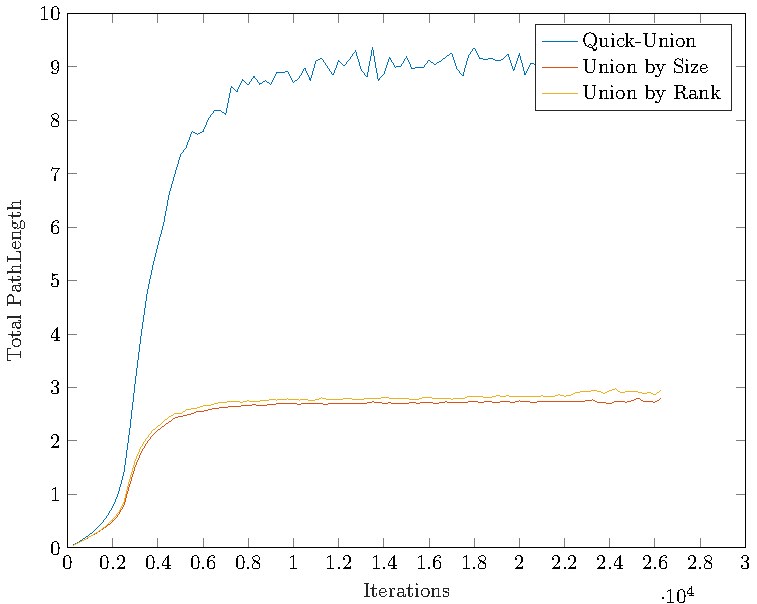
\includegraphics[width=\textwidth]{../images/plotTORFull5000_PathLength.pdf}
        \caption{Path Lengths with different union strategies with $n = 5000$ using Type One Reversal}
    \end{subfigure}%
    \hfill
    % Subfigure 3
    \begin{subfigure}{0.32\textwidth}
        \centering
        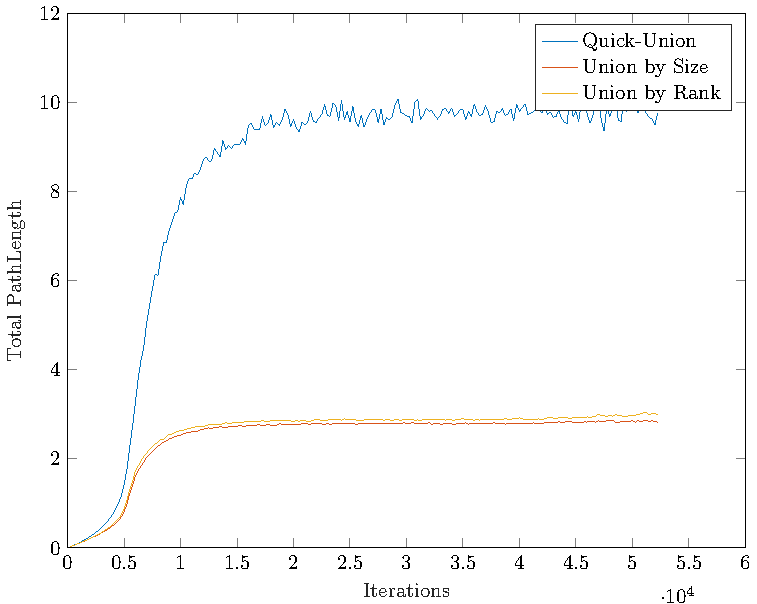
\includegraphics[width=\textwidth]{../images/plotTORFull10000_PathLength.pdf}
        \caption{Path Lengths with different union strategies with $n = 10000$ using Type One Reversal}
    \end{subfigure}

    \caption{Total Path Length normalized for different heuristics}
    \label{fig:tplH}
\end{figure}

\begin{figure}[ht]
    \centering
    \begin{subfigure}{0.32\textwidth}
        \centering
        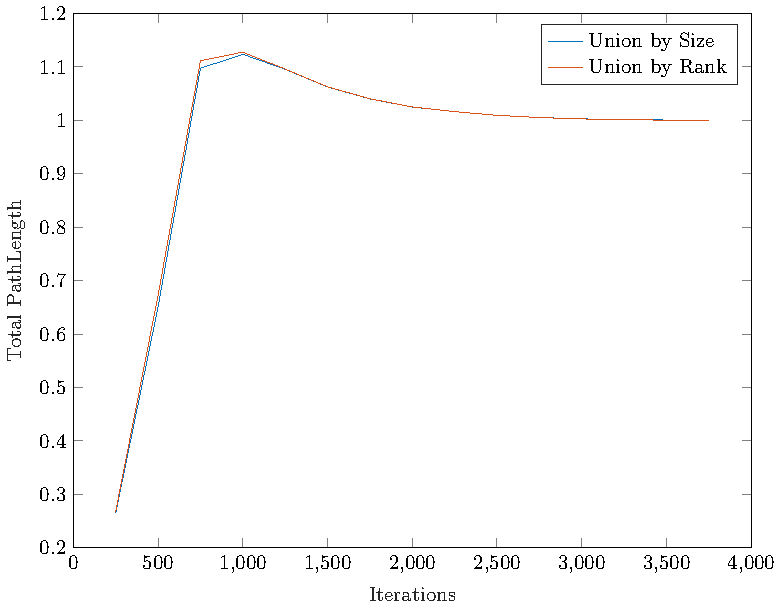
\includegraphics[width=\textwidth]{../images/plotFCNonFull1000_PathLength.pdf}
        \caption{Path Lengths with different union strategies with $n = 1000$ using Full Compression}
    \end{subfigure}%
    \hfill
    % Subfigure 2
    \begin{subfigure}{0.32\textwidth}
        \centering
        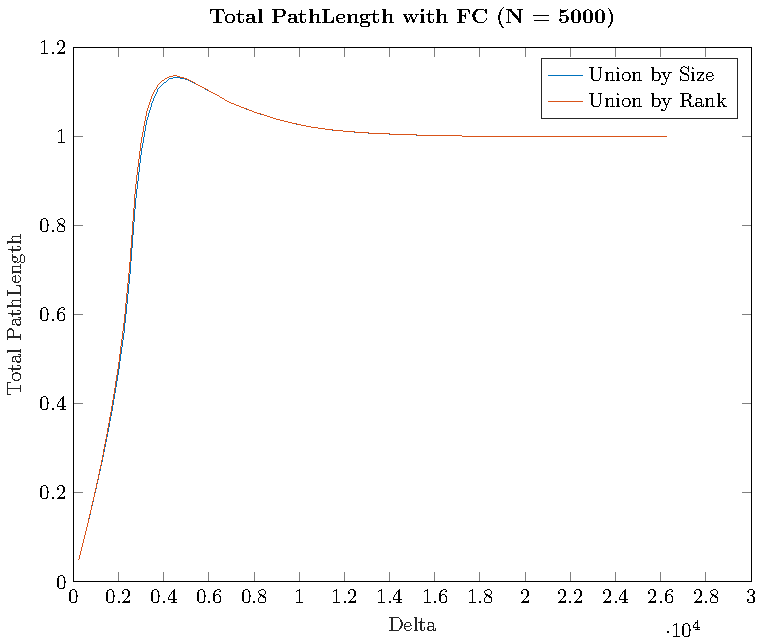
\includegraphics[width=\textwidth]{../images/plotFCNonFull5000_PathLength.pdf}
        \caption{Path Lengths with different union strategies with $n = 5000$ using Full Compression}
    \end{subfigure}%
    \hfill
    % Subfigure 3
    \begin{subfigure}{0.32\textwidth}
        \centering
        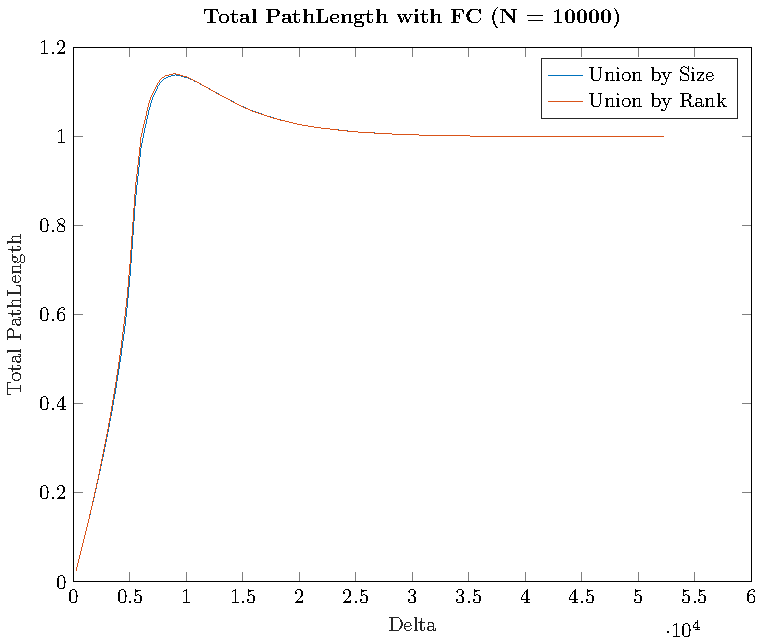
\includegraphics[width=\textwidth]{../images/plotFCNonFull10000_PathLength.pdf}
        \caption{Path Lengths with different union strategies with $n = 10000$ using Full Compression}
    \end{subfigure}
    % Subfigure 1
    \begin{subfigure}{0.32\textwidth}
        \centering
        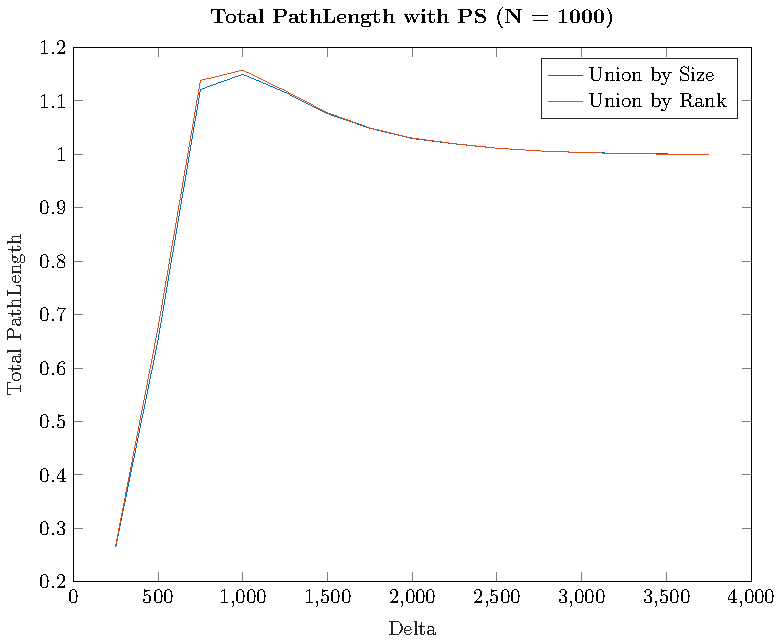
\includegraphics[width=\textwidth]{../images/plotPSNonFull1000_PathLength.pdf}
        \caption{Path Lengths with different union strategies with $n = 1000$ using Path Splitting}
    \end{subfigure}%
    \hfill
    % Subfigure 2
    \begin{subfigure}{0.32\textwidth}
        \centering
        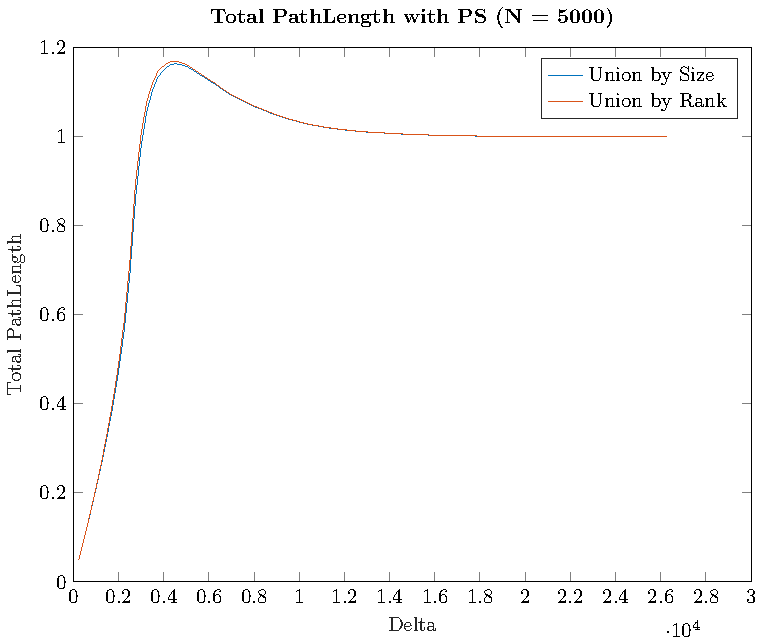
\includegraphics[width=\textwidth]{../images/plotPSNonFull5000_PathLength.pdf}
        \caption{Path Lengths with different union strategies with $n = 5000$ using Path Splitting}
    \end{subfigure}%
    \hfill
    % Subfigure 3
    \begin{subfigure}{0.32\textwidth}
        \centering
        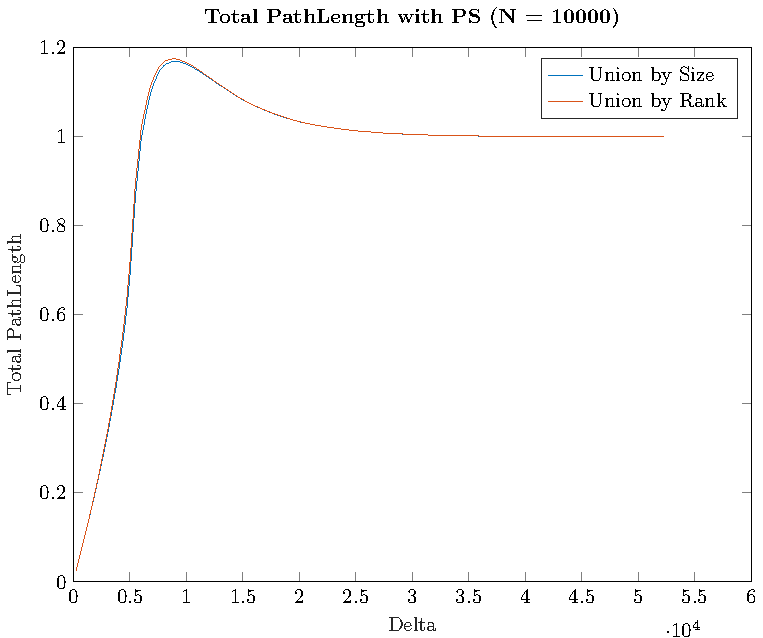
\includegraphics[width=\textwidth]{../images/plotPSNonFull10000_PathLength.pdf}
        \caption{Path Lengths with different union strategies with $n = 10000$ using Path Splitting}
    \end{subfigure}

    \begin{subfigure}{0.32\textwidth}
        \centering
        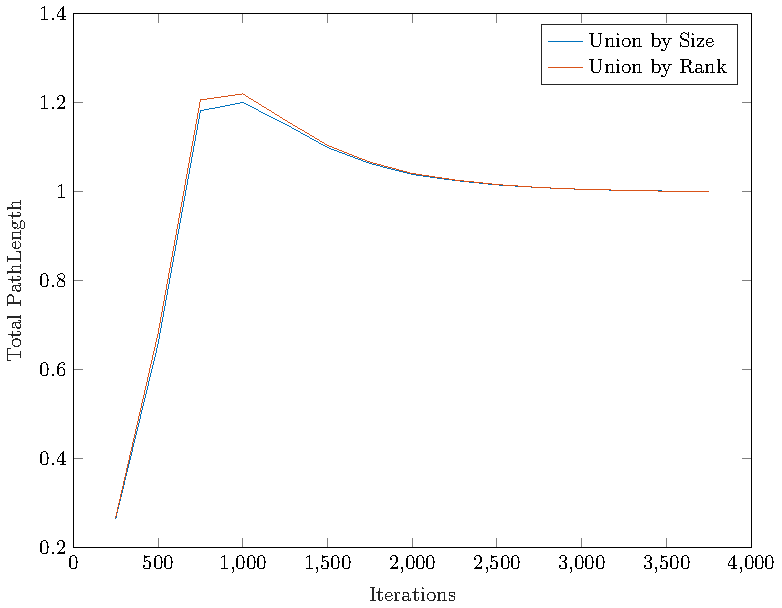
\includegraphics[width=\textwidth]{../images/plotPHNonFull1000_PathLength.pdf}
        \caption{Path Lengths with different union strategies with $n = 1000$ using Path Halving}
    \end{subfigure}%
    \hfill
    % Subfigure 2
    \begin{subfigure}{0.32\textwidth}
        \centering
        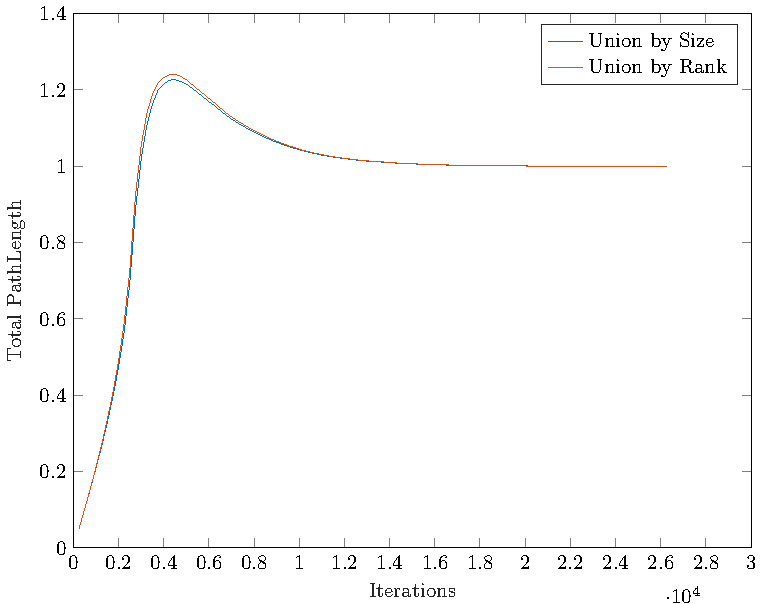
\includegraphics[width=\textwidth]{../images/plotPHNonFull5000_PathLength.pdf}
        \caption{Path Lengths with different union strategies with $n = 5000$ using Path Halving}
    \end{subfigure}%
    \hfill
    % Subfigure 3
    \begin{subfigure}{0.32\textwidth}
        \centering
        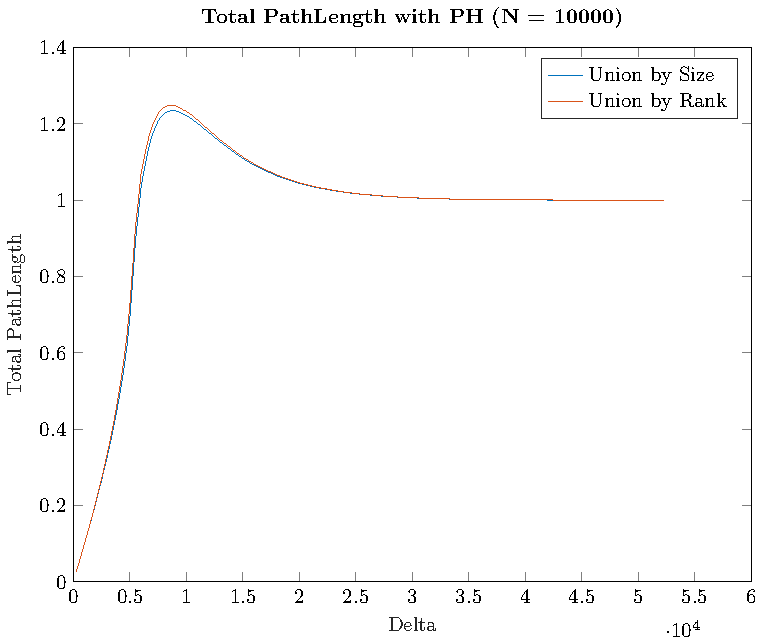
\includegraphics[width=\textwidth]{../images/plotPHNonFull10000_PathLength.pdf}
        \caption{Path Lengths with different union strategies with $n = 10000$ using Path Halving}
    \end{subfigure}
    \begin{subfigure}{0.32\textwidth}
        \centering
        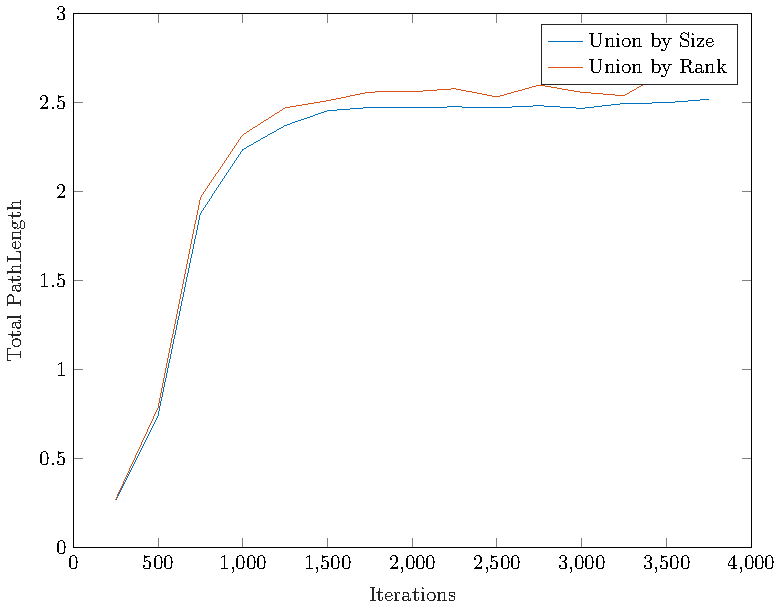
\includegraphics[width=\textwidth]{../images/plotTORNonFull1000_PathLength.pdf}
        \caption{Path Lengths with different union strategies with $n = 1000$ using Type One Reversal}
    \end{subfigure}%
    \hfill
    % Subfigure 2
    \begin{subfigure}{0.32\textwidth}
        \centering
        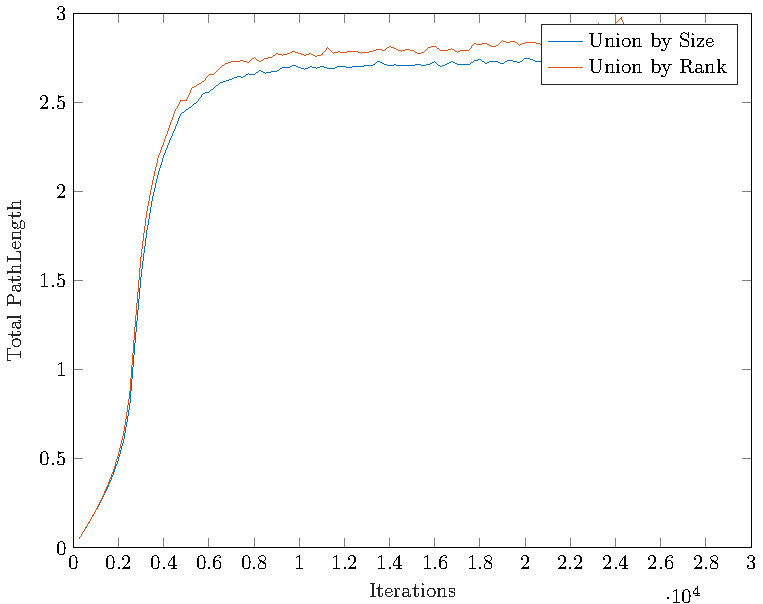
\includegraphics[width=\textwidth]{../images/plotTORNonFull5000_PathLength.pdf}
        \caption{Path Lengths with different union strategies with $n = 5000$ using Type One Reversal}
    \end{subfigure}%
    \hfill
    % Subfigure 3
    \begin{subfigure}{0.32\textwidth}
        \centering
        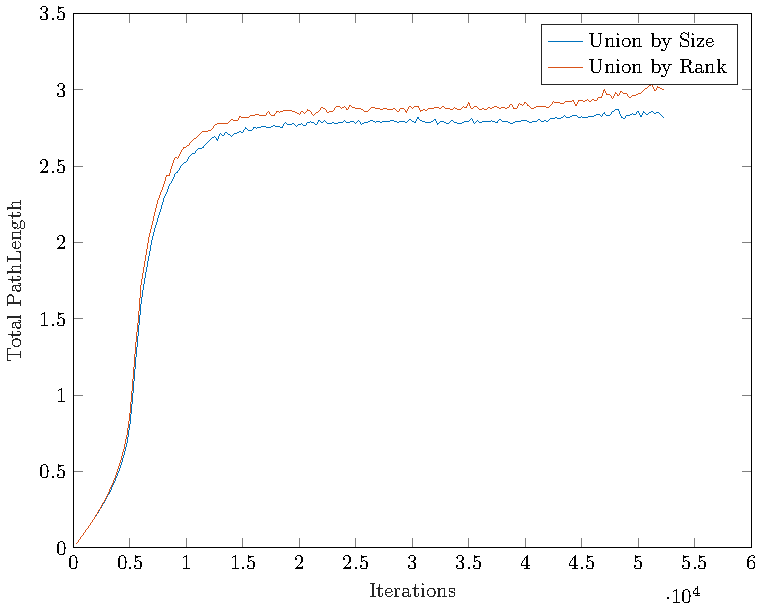
\includegraphics[width=\textwidth]{../images/plotTORNonFull10000_PathLength.pdf}
        \caption{Path Lengths with different union strategies with $n = 10000$ using Type One Reversal}
    \end{subfigure}

    \caption{Total Path Length normalized for different heuristics without Quick-Union}
    \label{fig:tplNH}
\end{figure}



\begin{figure}[ht]
    \centering
    \begin{subfigure}{0.32\textwidth}
        \centering
        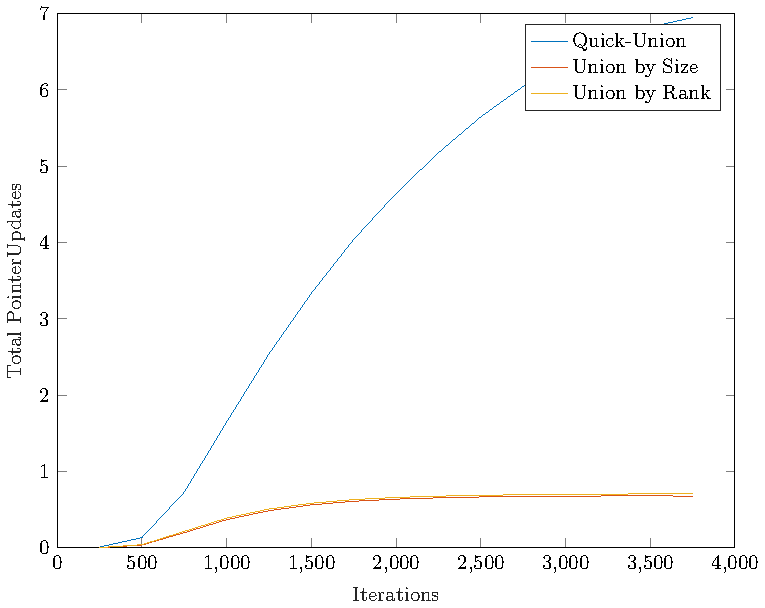
\includegraphics[width=\textwidth]{../images/plotFCFull1000_PointerUpdates.pdf}
        \caption{Pointer Updates with different union strategies with $n = 1000$ using Full Compression}
    \end{subfigure}%
    \hfill
    % Subfigure 2
    \begin{subfigure}{0.32\textwidth}
        \centering
        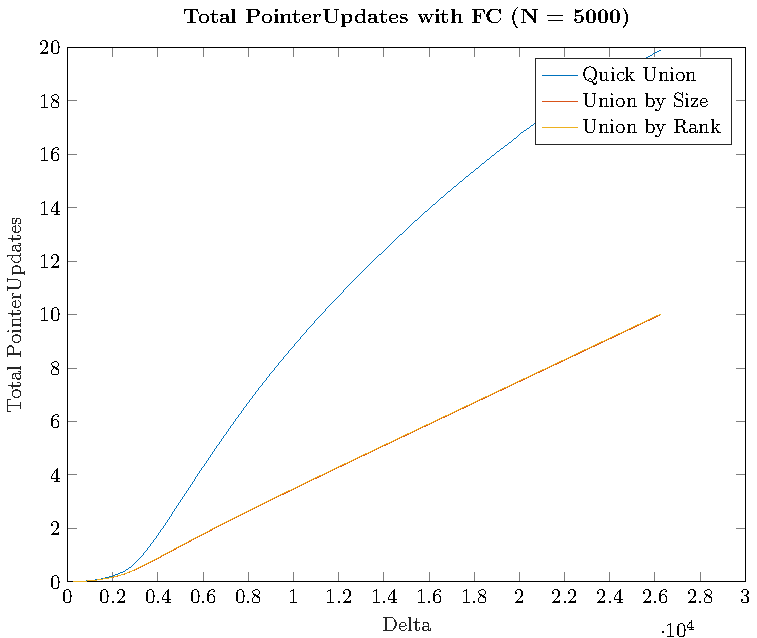
\includegraphics[width=\textwidth]{../images/plotFCFull5000_PointerUpdates.pdf}
        \caption{Pointer Updates with different union strategies with $n = 5000$ using Full Compression}
    \end{subfigure}%
    \hfill
    % Subfigure 3
    \begin{subfigure}{0.32\textwidth}
        \centering
        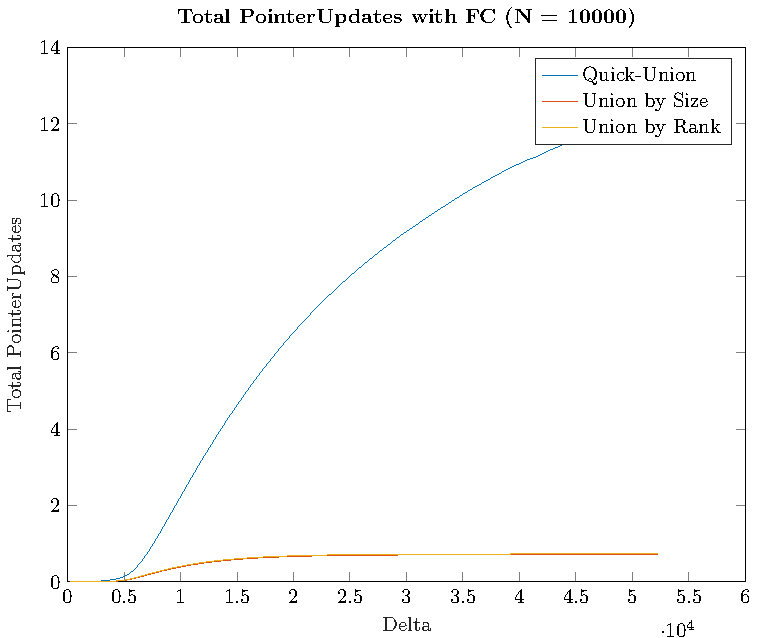
\includegraphics[width=\textwidth]{../images/plotFCFull10000_PointerUpdates.pdf}
        \caption{Pointer Updates with different union strategies with $n = 10000$ using Full Compression}
    \end{subfigure}
    % Subfigure 1
    \begin{subfigure}{0.32\textwidth}
        \centering
        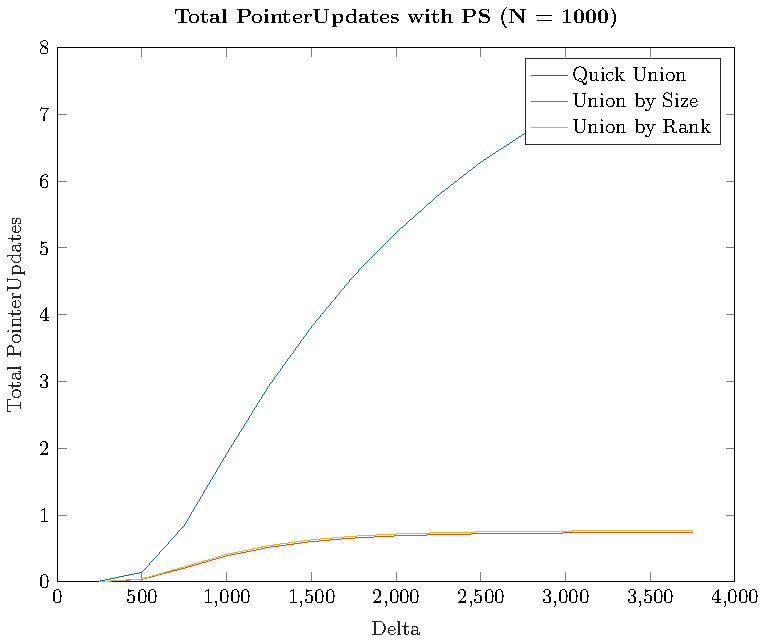
\includegraphics[width=\textwidth]{../images/plotPSFull1000_PointerUpdates.pdf}
        \caption{Pointer Updates with different union strategies with $n = 1000$ using Path Splitting}
    \end{subfigure}%
    \hfill
    % Subfigure 2
    \begin{subfigure}{0.32\textwidth}
        \centering
        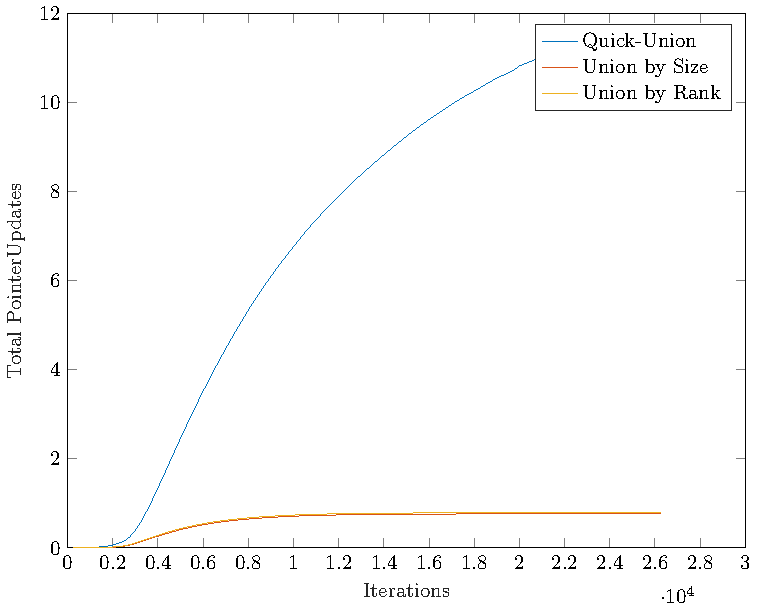
\includegraphics[width=\textwidth]{../images/plotPSFull5000_PointerUpdates.pdf}
        \caption{Pointer Updates with different union strategies with $n = 5000$ using Path Splitting}
    \end{subfigure}%
    \hfill
    % Subfigure 3
    \begin{subfigure}{0.32\textwidth}
        \centering
        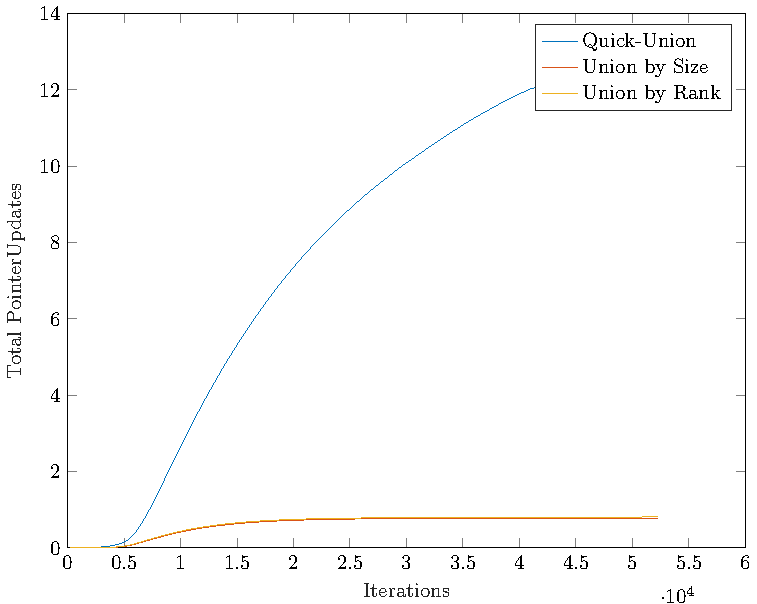
\includegraphics[width=\textwidth]{../images/plotPSFull10000_PointerUpdates.pdf}
        \caption{Pointer Updates with different union strategies with $n = 10000$ using Path Splitting}
    \end{subfigure}

    \begin{subfigure}{0.32\textwidth}
        \centering
        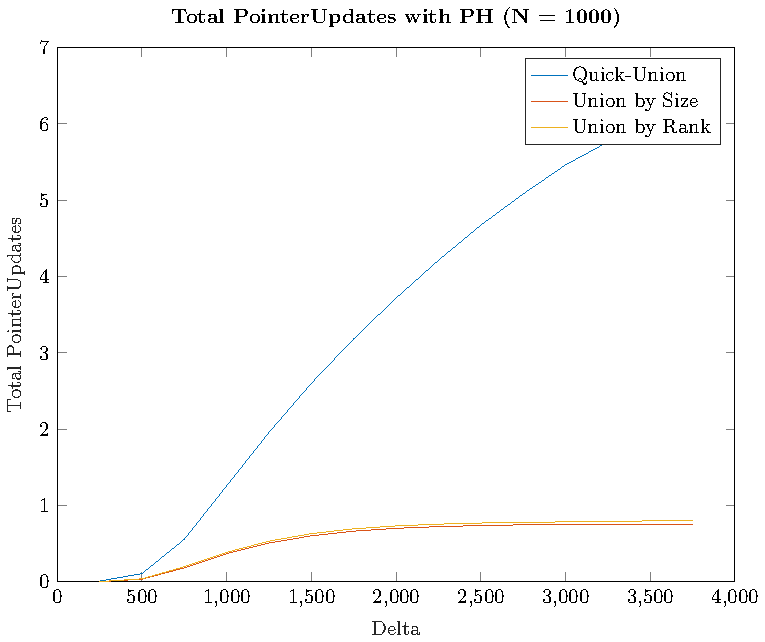
\includegraphics[width=\textwidth]{../images/plotPHFull1000_PointerUpdates.pdf}
        \caption{Pointer Updates with different union strategies with $n = 1000$ using Path Halving}
    \end{subfigure}%
    \hfill
    % Subfigure 2
    \begin{subfigure}{0.32\textwidth}
        \centering
        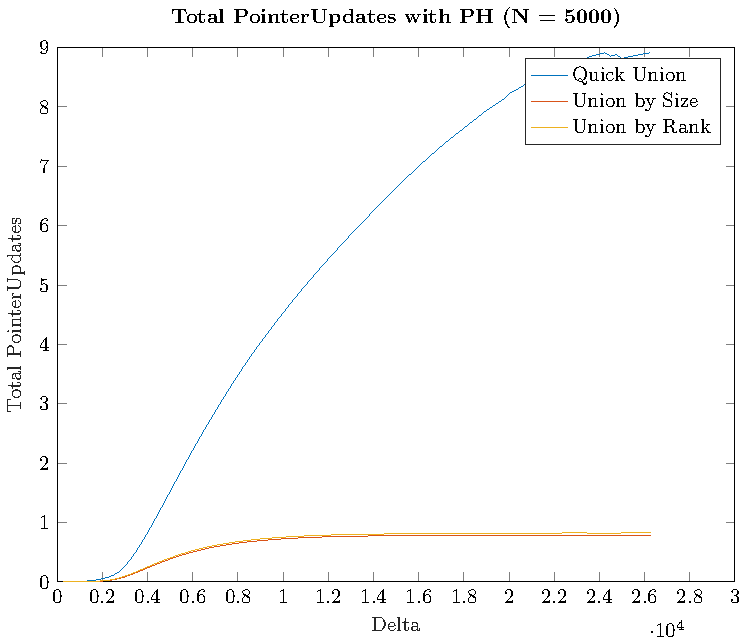
\includegraphics[width=\textwidth]{../images/plotPHFull5000_PointerUpdates.pdf}
        \caption{Pointer Updates with different union strategies with $n = 5000$ using Path Halving}
    \end{subfigure}%
    \hfill
    % Subfigure 3
    \begin{subfigure}{0.32\textwidth}
        \centering
        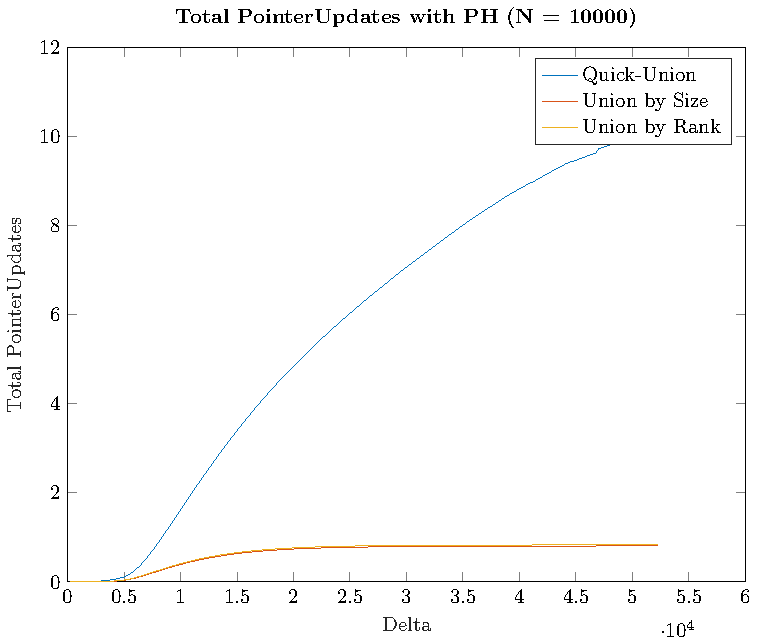
\includegraphics[width=\textwidth]{../images/plotPHFull10000_PointerUpdates.pdf}
        \caption{Pointer Updates with different union strategies with $n = 10000$ using Path Halving}
    \end{subfigure}

    \begin{subfigure}{0.32\textwidth}
        \centering
        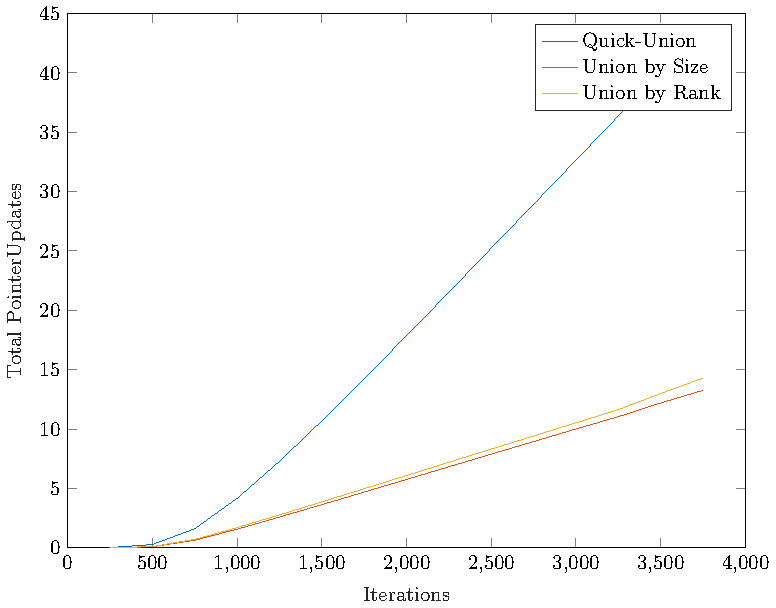
\includegraphics[width=\textwidth]{../images/plotTORFull1000_PointerUpdates.pdf}
        \caption{Pointer Updates with different union strategies with $n = 1000$ using Type One Reversal}
    \end{subfigure}%
    \hfill
    % Subfigure 2
    \begin{subfigure}{0.32\textwidth}
        \centering
        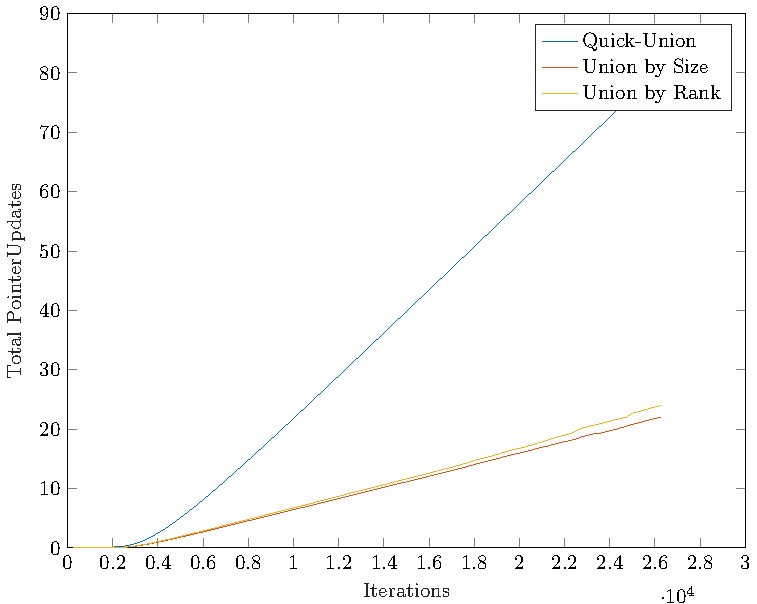
\includegraphics[width=\textwidth]{../images/plotTORFull5000_PointerUpdates.pdf}
        \caption{Pointer Updates with different union strategies with $n = 5000$ using Type One Reversal}
    \end{subfigure}%
    \hfill
    % Subfigure 3
    \begin{subfigure}{0.32\textwidth}
        \centering
        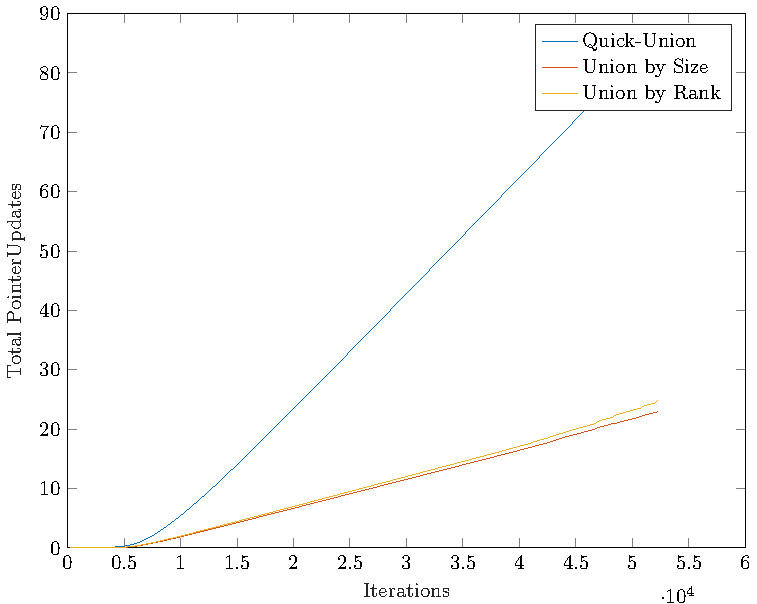
\includegraphics[width=\textwidth]{../images/plotTORFull10000_PointerUpdates.pdf}
        \caption{Pointer Updates with different union strategies with $n = 10000$ using Type One Reversal}
    \end{subfigure}

    \caption{Total Pointer Update normalized using different heuristics}
    \label{fig:tpuH}
\end{figure}


\begin{figure}[ht]
    \centering
    \begin{subfigure}{0.32\textwidth}
        \centering
        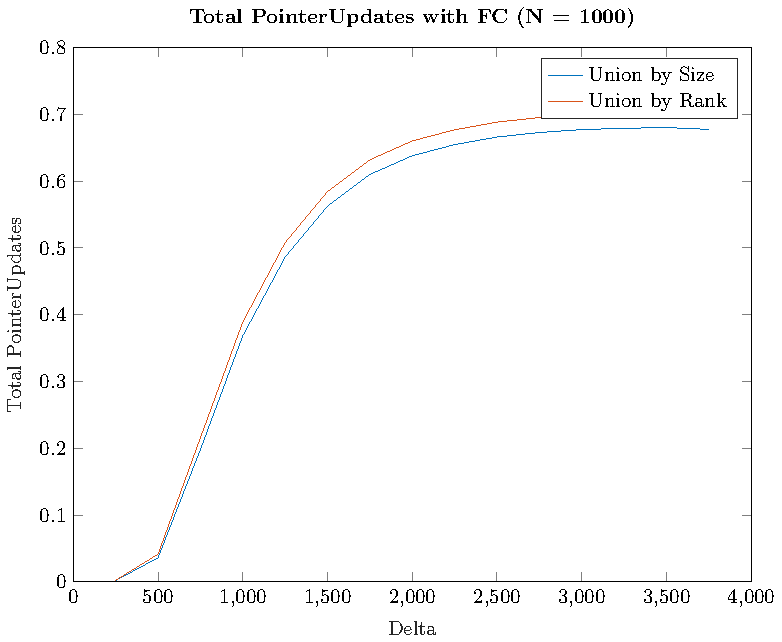
\includegraphics[width=\textwidth]{../images/plotFCNonFull1000_PointerUpdates.pdf}
        \caption{Pointer Updates with different union strategies with $n = 1000$ using Full Compression}
    \end{subfigure}%
    \hfill
    % Subfigure 2
    \begin{subfigure}{0.32\textwidth}
        \centering
        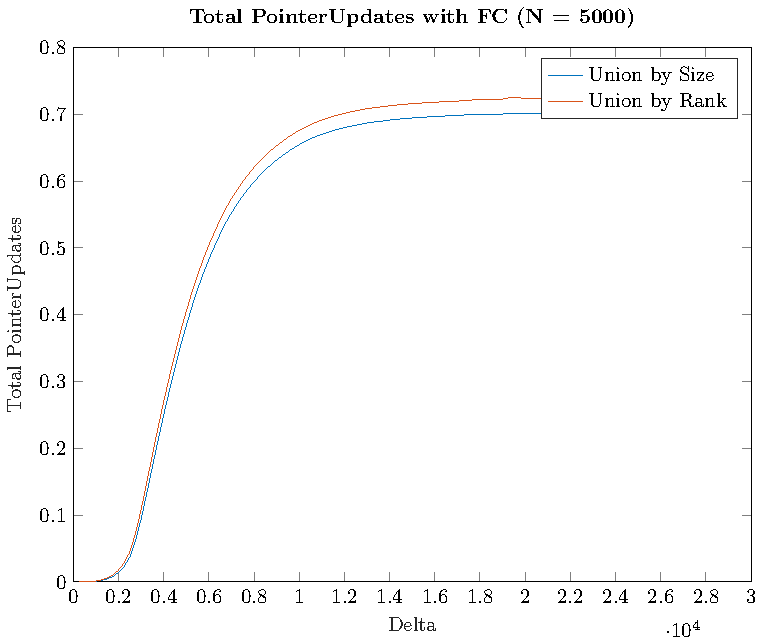
\includegraphics[width=\textwidth]{../images/plotFCNonFull5000_PointerUpdates.pdf}
        \caption{Pointer Updates with different union strategies with $n = 5000$ using Full Compression}
    \end{subfigure}%
    \hfill
    % Subfigure 3
    \begin{subfigure}{0.32\textwidth}
        \centering
        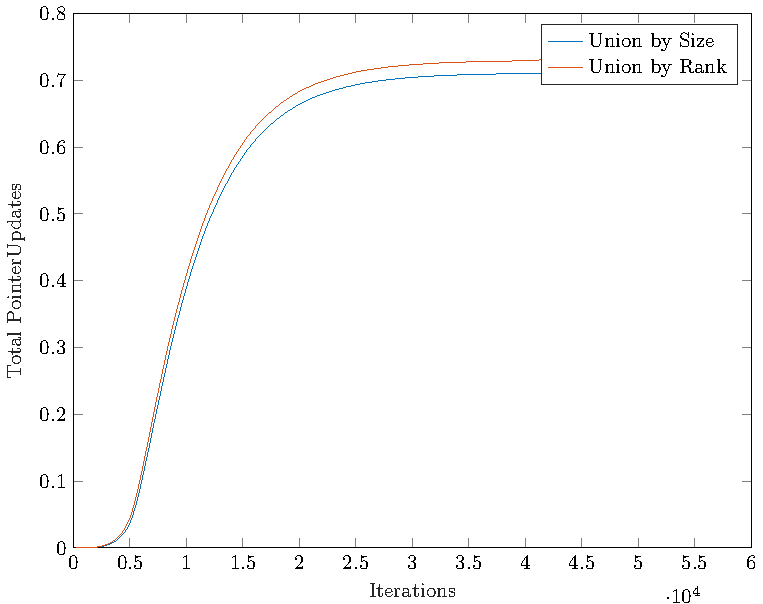
\includegraphics[width=\textwidth]{../images/plotFCNonFull10000_PointerUpdates.pdf}
        \caption{Pointer Updates with different union strategies with $n = 10000$ using Full Compression}
    \end{subfigure}
    % Subfigure 1
    \begin{subfigure}{0.32\textwidth}
        \centering
        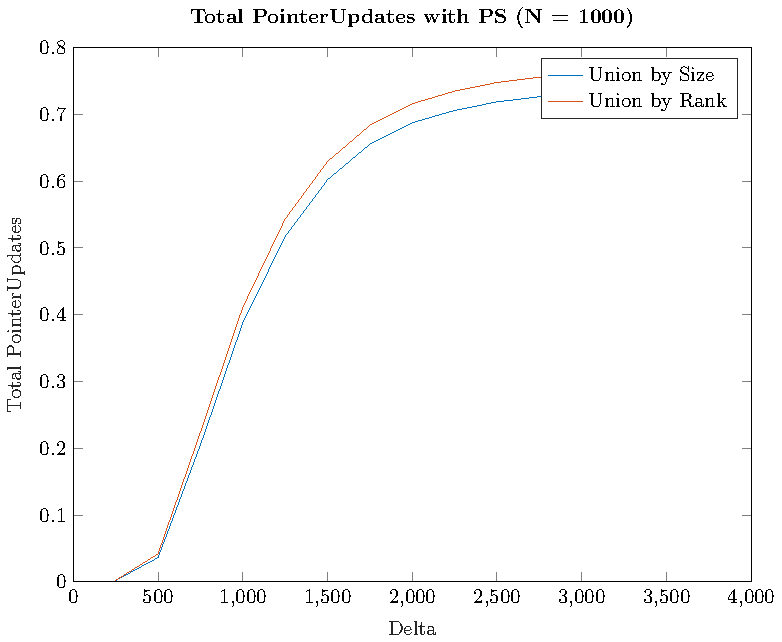
\includegraphics[width=\textwidth]{../images/plotPSNonFull1000_PointerUpdates.pdf}
        \caption{Pointer Updates with different union strategies with $n = 1000$ using Path Splitting}
    \end{subfigure}%
    \hfill
    % Subfigure 2
    \begin{subfigure}{0.32\textwidth}
        \centering
        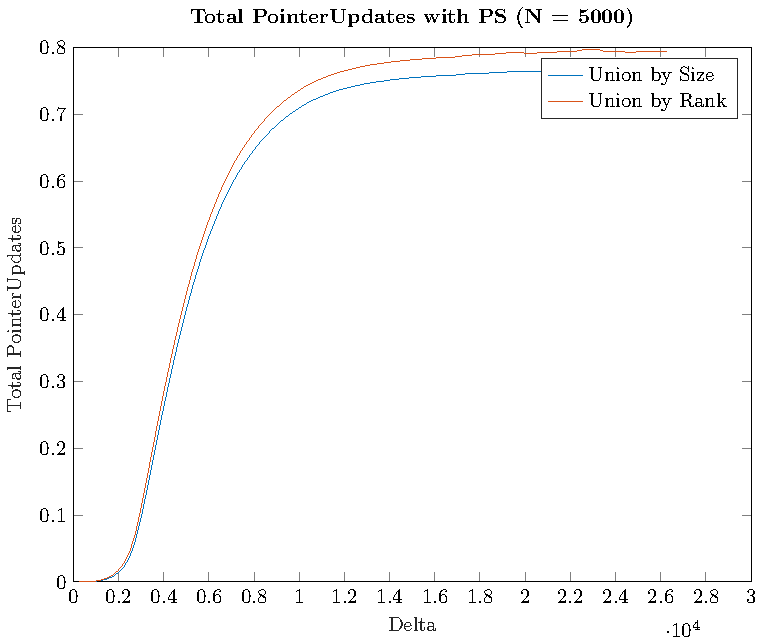
\includegraphics[width=\textwidth]{../images/plotPSNonFull5000_PointerUpdates.pdf}
        \caption{Pointer Updates with different union strategies with $n = 5000$ using Path Splitting}
    \end{subfigure}%
    \hfill
    % Subfigure 3
    \begin{subfigure}{0.32\textwidth}
        \centering
        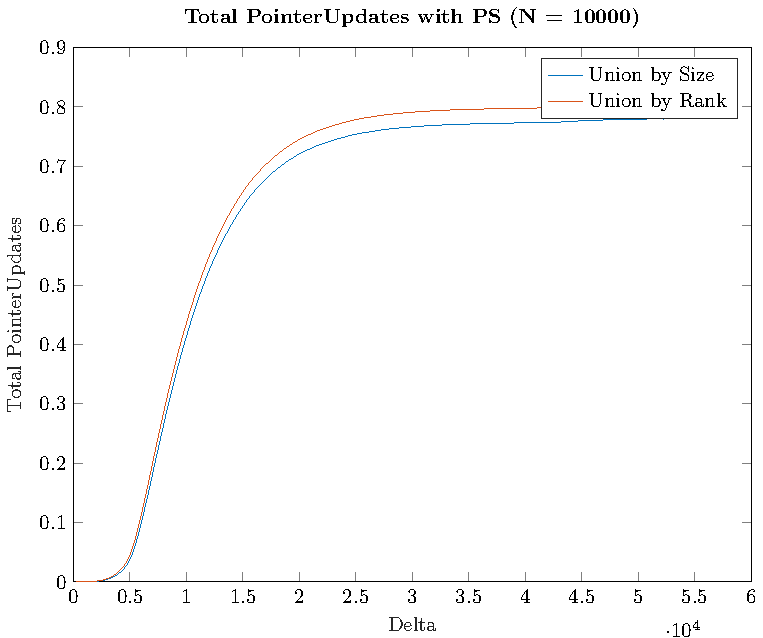
\includegraphics[width=\textwidth]{../images/plotPSNonFull10000_PointerUpdates.pdf}
        \caption{Pointer Updates with different union strategies with $n = 10000$ using Path Splitting}
    \end{subfigure}

    \begin{subfigure}{0.32\textwidth}
        \centering
        \includegraphics[width=\textwidth]{../images/plotPHNonFull1000_PointerUpdates.pdf}
        \caption{Pointer Updates with different union strategies with $n = 1000$ using Path Halving}
    \end{subfigure}%
    \hfill
    % Subfigure 2
    \begin{subfigure}{0.32\textwidth}
        \centering
        \includegraphics[width=\textwidth]{../images/plotPHNonFull5000_PointerUpdates.pdf}
        \caption{Pointer Updates with different union strategies with $n = 5000$ using Path Halving}
    \end{subfigure}%
    \hfill
    % Subfigure 3
    \begin{subfigure}{0.32\textwidth}
        \centering
        \includegraphics[width=\textwidth]{../images/plotPHNonFull10000_PointerUpdates.pdf}
        \caption{Pointer Updates with different union strategies with $n = 10000$ using Path Halving}
    \end{subfigure}

    \begin{subfigure}{0.32\textwidth}
        \centering
        \includegraphics[width=\textwidth]{../images/plotTORNonFull1000_PointerUpdates.pdf}
        \caption{Pointer Updates with different union strategies with $n = 1000$ using Type One Reversal}
    \end{subfigure}%
    \hfill
    % Subfigure 2
    \begin{subfigure}{0.32\textwidth}
        \centering
        \includegraphics[width=\textwidth]{../images/plotTORNonFull5000_PointerUpdates.pdf}
        \caption{Pointer Updates with different union strategies with $n = 5000$ using Type One Reversal}
    \end{subfigure}%
    \hfill
    % Subfigure 3
    \begin{subfigure}{0.32\textwidth}
        \centering
        \includegraphics[width=\textwidth]{../images/plotTORNonFull10000_PointerUpdates.pdf}
        \caption{Pointer Updates with different union strategies with $n = 10000$ using Type One Reversal}
    \end{subfigure}

    \caption{Total Pointer Update normalized without Quick-Union}
    \label{fig:tpuNH}
\end{figure}


